\section{Description of Datasets}
\label{sec:methods/section_a}

To our understanding, there is no public or open-source dataset of uncompressed video sequences with ground truths. Our group members prepared the uncompressed video sequences and annotated them to obtain ground truths in YOLO format. The existing ground truths prepared by our group members are suitable for object detection; however, for the purpose of analyzing the tracking performance, we further annotated the unique object identifier (ID) on the existing ground truths using Normalized Cross-correlation (NCC).
\begin{table}[htb]
    \centering
    \caption{List of Video Sequences adapted from \cite{choi_vcm_2020}}
    \resizebox{1.0\linewidth}{!}{
    \begin{tabular}{|| c | c | c | c | c | c | c ||}
         \hline
          Sequence Class & Sequence Name & Frame Count & Resolution & Object Class IDs & Frame rate (Hz) & Bit depth  \\ [0.5ex]
         \hline\hline
          B & BasketballDrive & 500 & 1920x1080 & [0, 32, 56] & 50 & 8 \\ 
         \hline
          B & Cactus & 500 & 1920x1080 & [58] & 50 & 8 \\ 
         \hline
          B & Kimono & 240 & 1920x1080 & [0, 26] & 24 & 8 \\
         \hline
          B & ParkScene & 240 & 1920x1080 & [0, 1, 13] & 24 & 8 \\
         \hline
          C & BasketballDrill & 500 & 832x480 & [0, 32, 56] & 50 & 8 \\
         \hline
          C & PartyScene & 500 & 832x480 & [0, 41, 58, 74, 77] & 50 & 8 \\
         \hline
          C & RaceHorses & 300 & 832x480 & [0, 17] & 30 & 8 \\
         \hline
          D & BasketballPass & 500 & 416x240 & [0, 32, 56] & 50 & 8 \\
         \hline
          D & BlowingBubbles & 500 & 416x240 & [0, 41, 77] & 50 & 8 \\
          \hline
          D & RaceHorses & 500 & 416x240 & [0, 17] & 30 & 8 \\
          \hline
          E & KristenAndSara & 600 & 1280x720 & [0, 63, 67] & 60 & 8 \\
          \hline
          E & Johnny & 600 & 1280x720 & [0, 27, 63] & 60 & 8 \\
          \hline
          E & FourPeople & 600 & 1280x720 & [0, 41, 56, 58] & 60 & 8 \\
          \hline
    \end{tabular}
    }
    \label{tab:seq_list}
\end{table}
Table \ref{tab:seq_list} shows the 13 uncompressed video sequences with prepared ground truths out of 18 available video sequences from \cite{choi_vcm_2020}. The sequence class (B, C, D, E) differs by the resolution (Width x Height). Each sequence has different number of object classes and each class ID is from 80 COCO object classes \cite{lin_microsoft_2014}. Table \ref{tab:class_id} adapted from \cite{choi_vcm_2020} shows the corresponding object class name to each class ID, and we only listed the object classes that we detect and track in the given sequences from Table \cite{tab:seq_list}.
\begin{table}[!htbp]
    \centering
    \caption{List of Object Class IDs adapted from \cite{choi_vcm_2020}}
    \resizebox{0.6\linewidth}{!}{
    \begin{tabular}{|| c | c | c | c ||}
         \hline
          Class ID & Object class name & Class ID & Object class name \\ [0.5ex]
         \hline\hline
          0 & Person & 41 & Cup \\
         \hline
          1 & Bicycle & 56 & Chair \\
         \hline
         13 & Bench & 58 & Potted plant \\
         \hline
         17 & Horse & 63 & Laptop \\
         \hline
         26 & Handbag & 67 & Cell phone \\
         \hline
         27 & Tie & 74 & Clock \\
         \hline
         32 & Sports ball & 77 & Teddy bear \\
         \hline
    \end{tabular}
    }
    \label{tab:class_id}
\end{table}
The uncompressed sequences are in YUV420 format. The object tracking pipeline consists of the YOLOv3 detector and SORT, as shown in Figure \ref{fig:yolov3+SORT}. 
\begin{figure}[!htbp]
  \centering
  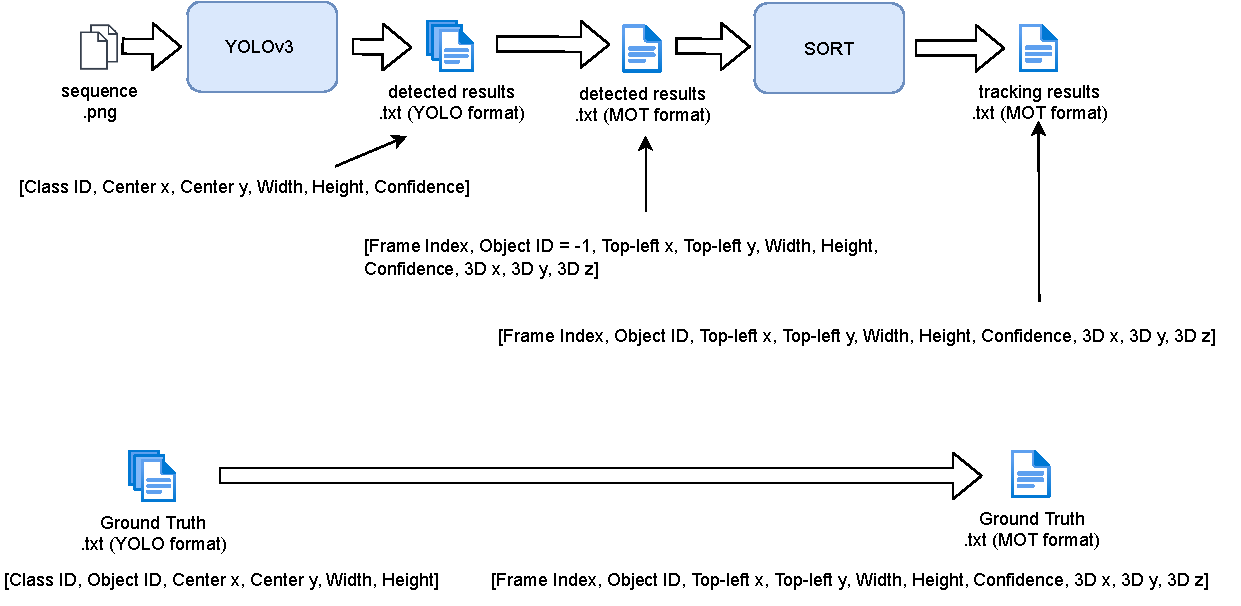
\includegraphics[width=1.0\linewidth]{img/YOLOv3+SORT.pdf}
  \caption[Object tracking pipeline with YOLO v3 and SORT]
  {Object tracking pipeline with YOLO v3 and SORT.}
  \label{fig:yolov3+SORT}
\end{figure}
Input video sequences of png files are input to the YOLOv3 object detector. The output from YOLOv3 as detected results will be generated in YOLO format as [Class ID, Center x, Center y, Width, Height, Confidence]. Class ID indicates the identifier to the type of object class; for example, "person" as 0, "sports ball" as 32, and "chair" as 56, which are part of the 80 COCO object classes. Center x and Center y are the center position of the bounding box; width and height are the corresponding dimensions of boxes; Confidence indicates the score of how confident the object is detected. These results are converted to the MOT format used in \textit{MOTChallenge} 2015 benchmark \cite{leal-taixe_motchallenge_2015}. The object ID, the unique identifier to the object, for the detected result is initialized as -1. Applying SORT to this detected result, we obtain the tracking result in MOT format with the assigned object ID as [Frame index, Object ID, Top-left x, Top-left y, Width, Height, Confidence, 3D x, 3D y, 3D z]. Top-left x and Top-left y are the positions of the bounding box at the top-left corner. 3D x, 3D y, 3D z is the bounding box position in 3D dimension, but we assigned -1 in our experiment since the 3-dimensional position is not applicable to our experiment. The ground truths are also converted from YOLO format to MOT format.

% The MOT format from \textit{MOTChallenge} is summarized in 
% \begin{myfont}
% \centering
% Class ID, Object ID, center X, center Y, Width, Height
% \end{myfont}


% \begin{table}[]
%     \centering
%     \caption{}
%     \begin{tabular}{|c|c|}
%         \hline
%         Data field & Description \\
%         \hline\hline
%         Frame Index & Frame index in a sequence \\
%         \hline
%         Object ID & Unique identifier to the object \\
%         \hline
%         Top-left x & x coordinate in top-left corner of the bounding box \\
%         \hline
%         Top-left y & y coordinate in top-left corner of the bounding box \\
%         \hline
%         Width & Width of the bounding box \\
%         \hline
%         Height & Height of the bounding box \\
%         \hline
%         Confidence & Confidence score of the detection of the object \\
%         \hline
%         3D x & x coordinate in 3D bounding box \\
%         \hline
%         3D y & y coordinate in 3D bounding box \\
%         \hline
%         3D z & z coordinate in 3D bounding box \\
%         \hline
%     \end{tabular}
%     \label{tab:MOT_format}
% \end{table}


